%%%%%%%%%%%%%%%%%%%%%%%%%%%%%%%%%%%%%%%%%%%%%%%%%%%%%%
%% Preámbulo de LaTeX para o caderno de exercicios %%%
%%%%%%%%%%%%%%%%%%%%%%%%%%%%%%%%%%%%%%%%%%%%%%%%%%%%%%
%
% Clase de documento:
\documentclass[a4papper,12pt,notitlepage,spanish]{article}
%
% Cargamos configuración
% ----------------------
% Seleccionar o idioma:
%%%%%%%%%%%%%%%%%%%%%%%%%%%%%%%%%%%%%%%%%%%
%% ---------- MODELO EJERCICIOS ---------- 
%% MATERIA: HISTORIA
%% CURSO: 
%% AÑO ACADÉMICO: 
%% CENTRO: 
%%%%%%%%%%%%%%%%%%%%%%%%%%%%%%%%%%%%%%%%%%%
%% 
%% MODELO PARA REDACTAR EJERCICIOS
%% ===============================
%% 
%% Clase de documento
%% ------------------
%\documentclass[letterpaper,12pt,notitlepage,spanish]{article}
%\documentclass[12pt,a4paper,notitlepage]{article}
%
% Márgenes de documento
% ---------------------
\usepackage[left=2.0cm, right=2.0cm, lines=45, top=2.5cm, bottom=2.0cm]{geometry}
%
% Paquetes necesarios
% -------------------
\usepackage[utf8]{inputenc} % acentos en ES
\usepackage[spanish,activeacute, es-tabla]{babel}
\usepackage{enumerate} % entornos de listas
\usepackage{multicol}  % varias columnas texto
\usepackage{fancyhdr}  % encabezado personalizado
\usepackage{fancybox}  % entornos con cajas
\usepackage{pdfpages}  % páginas pdf
%
\usepackage{lipsum} % generar texto aleatorio "loren ipsum"
\usepackage{environ} 
\usepackage{probsoln} % paquete para soluciones
%\showanswers % para mostrar soluciones
%
%Esto es lo importante. Ponemos la solución al margen.
\NewEnviron{solutionnew}{%
%  \leavevmode\marginpar{\raggedright\footnotesize \textbf{Solución:}\\ \BODY}
%  \textbf{Solución:}\\ \BODY} % sol. con salto de liña
  \small{Solución:} \BODY} % sol. na mesma liña
  {}
\renewenvironment{solution}{\solutionnew}{\endsolutionnew}
%
% FIGURAS EN COLUMNAS:
\newenvironment{Figura}
  {\par\medskip\noindent\minipage{\linewidth}}
  {\endminipage\par\medskip}
% ---
%
% Lineas de encabezado y pié
% --------------------------
\renewcommand{\headrulewidth}{0.5pt}
%\renewcommand{\headrulewidth}{1.0pt}
\renewcommand{\footrulewidth}{0.5pt}
%\renewcommand{\footrulewidth}{1.0pt}
\pagestyle{fancy} % estilo de página
%
% Recuadros y figuras
% -------------------
\newcommand\Loadedframemethod{TikZ}
\usepackage[framemethod=\Loadedframemethod]{mdframed}
\usepackage{tikz}
\usetikzlibrary{calc,through,backgrounds}
\usetikzlibrary{matrix,positioning}
%Desssins geometriques
\usetikzlibrary{arrows}
\usetikzlibrary{shapes.geometric}
\usetikzlibrary{datavisualization}
\usetikzlibrary{automata} % LATEX and plain TEX
\usetikzlibrary{shapes.multipart}
\usetikzlibrary{decorations.pathmorphing} 
\usepackage{pgfplots}
\usepackage{physics}
\usepackage{titletoc}
\usepackage{mathpazo} 
\usepackage{algpseudocode}
\usepackage{algorithmicx} 
\usepackage{bohr} 
\usepackage{xlop} 
\usepackage{bbding} 
%\usepackage{minibox} 
% Texto árabe
\usepackage{mathdesign}
\usepackage{bbding} 
% --
% Tipograía:
% ----------
% Fuente HEURÍSTICA (cómoda de leer)
%\usepackage{heuristica}
% Fuente LIBERTINE (cómoda para apuntes)
\usepackage{libertineRoman}
%\usepackage[proportional]{libertine}
% Fuente ROMANDE (estilo antiguo pero no muy cómoda)
%\usepackage{romande} %
% 
% Encabezado y pié de página (textos)
% -----------------------------------
% Modelo 1:
% ---------
% texto de encabezado izquierda:
%\lhead{\normalfont{Historia de la Música I}}
% texto encabezado centro:
%\chead{\textbf{Ejercicios}}
% texto de encabezado derecha:
%\rhead{\normalfont{curso: 2020/2021}}
% texto pié izquierdo:
%\lfoot{\small{\textit{}}}
% texto pié centrado:
%\cfoot{\textsc{Pág. \thepage }}
% texto pié derecho
%\rfoot{\textit{Pr. $\mathcal{A}$.Kaal}}
% ----------
% Modelo 2:
% ---------
% Encabezado y pié de página (textos)
% -----------------------------------
% texto de encabezado izquierda:
%
%\lhead{
%	\hrule
%	\vspace*{0.20cm}
%	\normalfont{Historia de la Música I}
%	\vspace*{0.10cm}
	%\hrule
%}
% texto encabezado centro:
%\chead{
%	\textbf{Cuestionario de Ejercicios}
%	\vspace*{0.08cm}}
% texto de encabezado derecha:
%\rhead{
%	\normalfont{curso: 2020/2021}
%	\vspace*{0.08cm}}
%
% texto pié izquierdo:
%\lfoot{
	%\begin{center}
		%\vspace*{0.20cm}
		%\hrule
		%\small{
		%Conservatorio Profesional de Música de Viveiro - Avda. da mariña s/n - (27850) Viveiro - Lugo
		%	}
	%\end{center}
%}
% texto pié centrado:
%\cfoot{
	%\vspace*{0.30cm}
	%\hrule
	%\vspace*{0.90cm}
%	\small{- Página \thepage -  }\\
	%\small{Conservatorio Profesional de Música de Viveiro}\\
	%\small{avda. da Mariña s/n}
%}

% ----------
% Modelo 3:
% ---------
% Encabezado y pié de página (textos)
% -----------------------------------
% texto de encabezado izquierda:
%
\lhead{
	\hrule
	\vspace*{0.20cm}
	\normalfont{Historia da Música I}
	\vspace*{0.10cm}
	%\hrule
}
% texto encabezado centro:
\chead{
	\textbf{CADERNO DE EXERCICIOS}
	\vspace*{0.08cm}}
% texto de encabezado derecha:
\rhead{
	\normalfont{curso: 2021/2022}
	\vspace*{0.08cm}}
%
% texto pié izquierdo:
%\lfoot{
	%\begin{center}
		%\vspace*{0.20cm}
		%\hrule
		%\small{
		%Conservatorio Profesional de Música de Viveiro - Avda. da mariña s/n - (27850) Viveiro - Lugo
		%	}
	%\end{center}
%}
% texto pié centrado:
\cfoot{
	%\vspace*{0.30cm}
	%\hrule
	%\vspace*{0.90cm}
	\small{- \thepage -  }\\
	%\small{Conservatorio Profesional de Música de Viveiro}\\
	%\small{avda. da Mariña s/n}
}

% --------
%=====================Algo setup
\algblock{If}{EndIf}
\algcblock[If]{If}{ElsIf}{EndIf}
\algcblock{If}{Else}{EndIf}
\algrenewtext{If}{\textbf{si}}
\algrenewtext{Else}{\textbf{sinon}}
\algrenewtext{EndIf}{\textbf{finsi}}
\algrenewtext{Then}{\textbf{alors}}
\algrenewtext{While}{\textbf{tant que}}
\algrenewtext{EndWhile}{\textbf{fin tant que}}
\algrenewtext{Repeat}{\textbf{r\'ep\'eter}}
\algrenewtext{Until}{\textbf{jusqu'\`a}}
\algcblockdefx[Strange]{If}{Eeee}{Oooo}
[1]{\textbf{Eeee} "#1"}
{\textbf{Wuuuups\dots}}

\algrenewcommand\algorithmicwhile{\textbf{TantQue}}
\algrenewcommand\algorithmicdo{\textbf{Faire}}
\algrenewcommand\algorithmicend{\textbf{Fin}}
\algrenewcommand\algorithmicrequire{\textbf{Variables}}
\algrenewcommand\algorithmicensure{\textbf{Constante}}% replace ensure by constante
\algblock[block]{Begin}{End}
\newcommand\algo[1]{\textbf{algorithme} #1;}
\newcommand\vars{\textbf{variables } }
\newcommand\consts{\textbf{constantes}}
\algrenewtext{Begin}{\textbf{debut}}
\algrenewtext{End}{\textbf{fin}}
%================================
%================================

\setlength{\parskip}{1.25cm}
\setlength{\parindent}{1.25cm}
\tikzstyle{titregris} =
[draw=gray,fill=gray, shading = exersicetitle, %
text=gray, rectangle, rounded corners, right,minimum height=.3cm]
\pgfdeclarehorizontalshading{exersicebackground}{100bp}
{color(0bp)=(green!40); color(100bp)=(black!5)}
\pgfdeclarehorizontalshading{exersicetitle}{100bp}
{color(0bp)=(red!40);color(100bp)=(black!5)}
\newcounter{exercise}
%\renewcommand*\theexercise{exercice \textbf{Ejercicio}~n\arabic{exercise}} % CASTELÁN
\renewcommand*\theexercise{exercice \textbf{Exercicio}~n\arabic{exercise}} % GALEGO
\makeatletter
\def\mdf@@exercisepoints{}%new mdframed key:
\define@key{mdf}{exercisepoints}{%
\def\mdf@@exercisepoints{#1}
}
\mdfdefinestyle{exercisestyle}{%
outerlinewidth=1em,outerlinecolor=white,%
leftmargin=-1em,rightmargin=-1em,%
middlelinewidth=0.5pt,roundcorner=3pt,linecolor=black,
apptotikzsetting={\tikzset{mdfbackground/.append style ={%
shading = exersicebackground}}},
innertopmargin=0.1\baselineskip,
skipabove={\dimexpr0.1\baselineskip+0\topskip\relax},
skipbelow={-0.1em},
needspace=0.5\baselineskip,
frametitlefont=\sffamily\bfseries,
settings={\global\stepcounter{exercise}},
singleextra={%
\node[titregris,xshift=0.5cm] at (P-|O) %
{~\mdf@frametitlefont{\theexercise}~};
\ifdefempty{\mdf@@exercisepoints}%
{}%
{\node[titregris,left,xshift=-1cm] at (P)%
{~\mdf@frametitlefont{\mdf@@exercisepoints points}~};}%
},
firstextra={%
\node[titregris,xshift=1cm] at (P-|O) %
{~\mdf@frametitlefont{\theexercise}~};
\ifdefempty{\mdf@@exercisepoints}%
{}%
{\node[titregris,left,xshift=-1cm] at (P)%
{~\mdf@frametitlefont{\mdf@@exercisepoints points}~};}%
},
}
\makeatother


%%%%%%%%%

%%%%%%%%%%%%%%%
\mdfdefinestyle{theoremstyle}{%
outerlinewidth=0.01em,linecolor=black,middlelinewidth=0.5pt,%
frametitlerule=true,roundcorner=2pt,%
apptotikzsetting={\tikzset{mfframetitlebackground/.append style={%
shade,left color=white, right color=blue!20}}},
frametitlerulecolor=black,innertopmargin=1\baselineskip,%green!60,
innerbottommargin=0.5\baselineskip,
frametitlerulewidth=0.1pt,
innertopmargin=0.7\topskip,skipabove={\dimexpr0.2\baselineskip+0.1\topskip\relax},
frametitleaboveskip=1pt,
frametitlebelowskip=1pt
}
\setlength{\parskip}{0mm}
\setlength{\parindent}{10mm}
%\mdtheorem[style=theoremstyle]{ejercicio}{\textbf{Ejercicio}} % Castelán
\mdtheorem[style=theoremstyle]{ejercicio}{\textbf{Exercicio}} % Galego
%================Liste definition--numList-and alphList=============
\newcounter{alphListCounter}
\newenvironment
{alphList}
{\begin{list}
{\alph{alphListCounter})}
{\usecounter{alphListCounter}
\setlength{\rightmargin}{0cm}
\setlength{\leftmargin}{0.5cm}
\setlength{\itemsep}{0.2cm}
\setlength{\partopsep}{0cm}
\setlength{\parsep}{0cm}}
}
{\end{list}}
\newcounter{numListCounter}
\newenvironment
{numList}
{\begin{list}
{\arabic{numListCounter})}
{\usecounter{numListCounter}
\setlength{\rightmargin}{0cm}
\setlength{\leftmargin}{0.5cm}
\setlength{\itemsep}{0cm}
\setlength{\partopsep}{0cm}
\setlength{\parsep}{0cm}}
}
{\end{list}}
%
%
%% -- Fin del archivo de configuración  --
%% % Galego
%\input{../../Modelos/include/config-HM1ejercicios_ES.tex} % Castelán
% --------------------------------
\usepackage{graphicx} % gráficos
\usepackage{hyperref} % enlaces
\usepackage{wrapfig} % figuras con textos
% \usepackage{chronology} % liñas de tempo
\usepackage{schemata} % para esquemas
\newcommand\diagram[2]{\schema{\schemabox{#1}}{\schemabox{#2}}}

% Directorio raíz de imaxes por defecto:
% --------------------------------------
% As imaxes son as mesmas que se usan no temario, polo que están nas carpetas de unidades correspondentes:
% P.Ex: /ud-00/figura.png

\graphicspath{ {../../../figures/} } %
%
% INICIO DO DOCUMENTO
% ===================

\begin{document}
% --------------------------------------------------
% Cargamos os exercicios desde o Banco de Exercicios
% -------------------------------------------------- 
% 
\hideanswers % oculta respostas
%
% Carga aquí os exercicios que correspondan a incluir na folla:
% -------------------------------------------------------------
% Espazo para cargar os exercicios predefinidos para exame
% ruta: actividades>cuestions
% -------------------------------------------------------------
%
% TÍTULO A FOLLA DE ACTIVIDADES:
%
\begin{center}
\Large{
1º Trimestre
} \\
\vspace*{0.5cm}
%
% DATOS DO ALUMNADO:
% -----------------
\vspace{1.10cm}
	\begin{flushleft}
	Nome e Apelidos: \hrulefill\\
	%\vspace*{0.50cm}
%
% INSTRUCCIÓNS:
% ------------
%		\begin{center}
%		\small{Instrucciones para realizar los ejercicios}\\		
%		\end{center}
%	\hrulefill \\
	%\vspace*{0.25cm}
%
%\small{ % INSTRUCCIONES:
%\texttt{Lee con atención y realiza con detenimiento, los siguientes ejercicios teniendo en cuenta lo que se indica en cada uno. \\
%}} % fin instrucciones.
%
	\vspace*{0.25cm}		
 	\end{flushleft}
\end{center}
\vspace*{1.10cm}
%

% ------------------------------------------  
% ACTIVIDADES.
% ------------------------------------------

% ACTIVIDADE 1.- (sobre tema 0)
%
% 
% EXERCICIOS DO TEMA 0.- INTRODUCCIÓN
%
% Repaso de conceptos de Perspectivas sobre a música

\section{Pensamentos, teorías e perspectivas sobre a música}

\begin{ejercicio}[Perspectivas sobre música- Rene Descartes]

% Ilustramos os exercicios con figuras
% --- Rene Descartes:
\begin{wrapfigure}{l}{0.30\textwidth} 
\begin{center} 
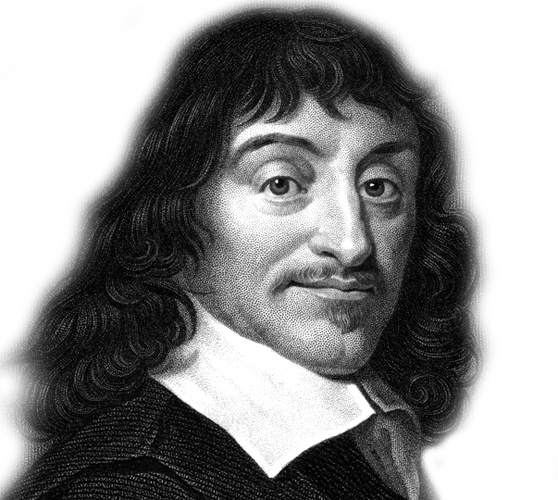
\includegraphics[width=0.20\textwidth]{/ud-00/descartes.png} 
\end{center} 
\caption{\\ \textbf{Rene Descartes} \\ 
Francia, 1596 - Suecia, 1650} 
\label{fig:descartes}
\end{wrapfigure}
% ---

As perspectivas sobre a música varian ao longo das diferentes épocas da historia. 
Algunhas reflexións, convidan a pensar na música como unha arte totalmente ligada a expresión de sentimentos; outras xustifican que, a música hai que considerala unha ciencia.

Desde os inicios da música, os teóricos, filósofos, músicos e grandes ilustrados trataron de comprender o feito musical e establecer relacións que lles axudasen a coñecer mellor o seu significado. É o caso de Pitágoras, Descartes, Kant, Wagner e moitos outros, que coas súas reflexións e perspectivas sobre a música sentan os precedentes do pensamento estétilo e musical, dentro da Historia do pensamento musical. 

Descartes s. {\scriptsize  XVII} define a música do seguinte xeito:

    \begin{quotation}{\small
     \noindent
     A mesma cousa que a uns invita a bailar a outros pode facer chorar. Pois isto non provén senón da asociación de ideas na nosa mente; como aqueles que algunha vez se divertiron bailando con certa peza, tan pronto como a volvan a escoltar volverán ás ganas de bailar; pola contra, se algún só oíu gallardas cando lle aconteceu algo malo, volverá  a entristecerse cando as escoite de novo.}
    \end{quotation}
 
\begin{enumerate}[1)]
 \item 
 Que perspectiva sobre a música adoita Descartes segundo a afirmación anterior?
 \begin{enumerate}[a)]
  \item 
  Música como expresión dos sentimentos
  \item
  Música como arte
  \item %\label{sol:1}
  Música como feito musical
  \item
  Ningunha das anteriores
 \end{enumerate}
 \item 
 A quen atribúes a seguinte afirmación? \dotfill
     \begin{quote}
    {\small
    Os números son as cousas; agora ben, a música é número. O mundo é música; o cosmos é unha lira sublime de sete cordas.
    }
    \end{quote}
\end{enumerate}

\end{ejercicio}

% --------------------------

\begin{ejercicio}[Perspectivas sobre música - Richard Wagner]

% Ilustramos os exercicios con figuras
% --- Richard Wagner:
\begin{wrapfigure}{r}{0.30\textwidth} 
\begin{center} 
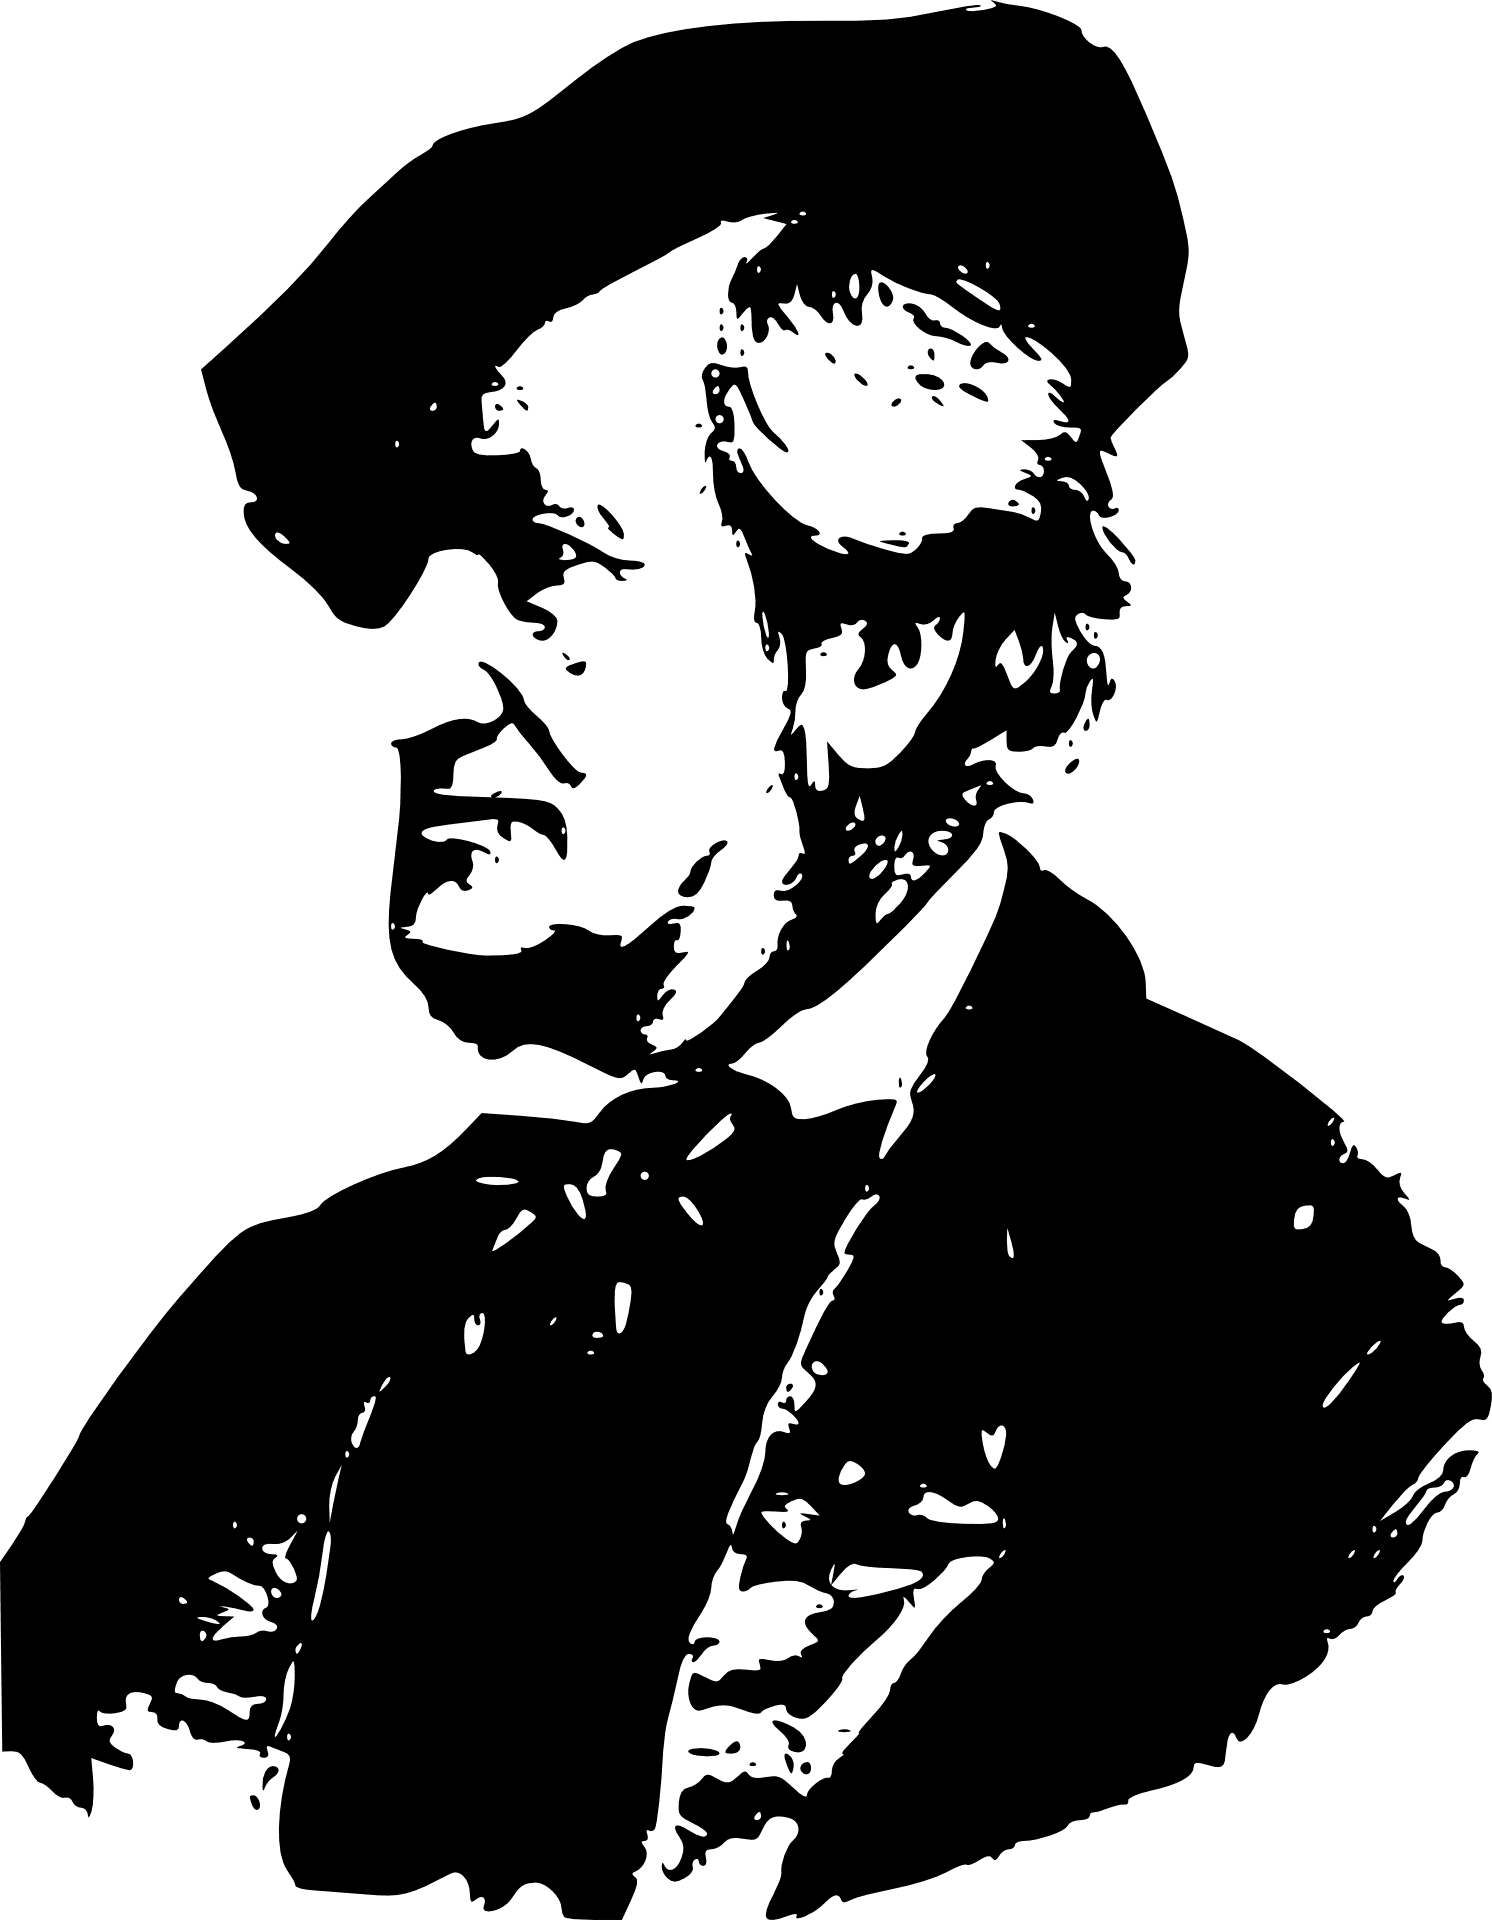
\includegraphics[width=0.20\textwidth]{/ud-00/wagner.png} 
\end{center} 
\caption{\\ \textbf{Richard Wagner} \\ 
Leipzig, 1813 - Venecia, 1883} 
\label{fig:wagner}
\end{wrapfigure}
% ---

Wilhelm Richard Wagner (Leipzig, 22 de maio de 1813 - Venecia, 13 de febreiro de 1883) foi un compositor, director de orquestra, poeta, ensaísta, dramaturgo e teórico musical alemán do Romanticismo.

Unha das súas maiores achegas á música foi o cambio de perspectiva acerca das composicións, que Wagner consideraba como ``obras de arte totais'' nas que sintetizaban todas as grandes artes: visuais, poéticas, escénicas, musicais, \ldots

Foi un dos máximos expoñentes do romanticismo musical alemán, que rompeu cos moldes canónicos do clasicismo. 
No s.{\scriptsize XIX}, Richard Wagner afirmaba sobre a música:

    \begin{quotation}{\small
     \noindent
     O son vén do corazón e a súa linguaxe artística natural é a música. A melodía é a lingua absoluta, a través da que o músico fala a todos os corazóns.}
    \end{quotation}
 
\begin{enumerate}[1)]
 \item 
 Que perspectiva sobre a música adoita Wagner segundo a afirmación anterior?
 \begin{enumerate}[a)]
  \item 
  Música como expresión dos sentimentos
  \item %\label{sol:2}
  Música como arte
  \item 
  Música como feito musical
  \item
  Ningunha das anteriores
 \end{enumerate}
 \item 
 A quen atribúes a seguinte afirmación sobre a música? \dotfill
     \begin{quote}
    {%\small
    [\ldots] a arte educativa por excelencia que se insire na alma e forma a virtude
    }
    \end{quote}
\end{enumerate}
\end{ejercicio}

% ------

\begin{ejercicio}[Teorías sobre a orixe da música]
Sinala a opción correcta, segundo as afirmacións que se indican nos seguintes puntos.
\begin{enumerate}[1)]
 \item 
 As teorías logoxénicas consideran que a música naceu asociada á linguaxe comunicativa.
  \begin{enumerate}[a)]
   \item %\label{sol:3}
   verdadeiro, nace da necesidade de comunicación
   \item 
   falso, tiñan unha función máxico-relixiosa
  \end{enumerate}
  \item
  Que teorías postulan que o corpo humano é un instrumento en si mesmo? 
  \begin{enumerate}[a)]
   \item 
   teorías logoxénicas
   \item 
   teorías máxico-relixiosas
   \item %\label{sol:4}
   teorías quinéticas
   \item 
   teorías conspirativas
  \end{enumerate}
 \end{enumerate}

\end{ejercicio}




\newpage
%
% ACTIVIDADE 2.- 
%
% 
% EXERCICIOS DO TEMA 0.- INTRODUCCIÓN - 
% Conceptos sobre a forma, xéneros musicais e estilos
%
% Repaso de conceptos de xeneros e formas da música

\begin{multicols}{2}

% EXERCICIO: FORMAS E ESTILOS
% ---------------------------
\begin{ejercicio}[Formas e estilos]
 \begin{enumerate}[1)]
  \item 
  Se nunha audición, analizamos os instrumentos que escoitamos nunha composición musical, en que aspecto estamos a fixar a nosa atención?

  \begin{enumerate}[a)]
   \item 
   Na textura
   \item % solución correcta
   No timbre
   \item
   Na forma
   \item
   No ritmo
  
  \end{enumerate}
  
  \item
   Cando escoitamos unha audición e tratamos de identificar a estrutura que ten, partes ou movementos, estamos a analizar a súa \ldots
  
  \begin{enumerate}[a)]
   \item 
   Textura
   \item 
   Timbre
   \item % solución correcta
   Forma
   \item
   Ritmo
  \end{enumerate}
 
 \end{enumerate}

\end{ejercicio}



% Repaso de conceptos de xeneros e formas da música
%\begin{multicols}{2}

% EXERCICIO: FONTES DE INFORMACIÓN
% --------------------------------

\begin{ejercicio}[Fontes de información]
 \begin{enumerate}[1)]
  \item 
  Indica cales son as principais fontes de información que consideramos no estudo da Historia da Música.

  \begin{enumerate}[1.]
   \item \dotfill 
   \item \dotfill 
   \item \dotfill 
   \item \dotfill 
  \end{enumerate}
 
 \item
 As pinturas, esculturas e outras obras de arte son consideradas fontes de información \par
 \dotfill
 \par
 Que é para ti unha fonte de información histórica?
 \par \vspace*{2.3cm}
 \end{enumerate}
\end{ejercicio}
%
\end{multicols}

% EXERCICIO: Liña temporal da historia
% ------------------------------------

\begin{ejercicio}[Liña temporal da historia]
 \begin{enumerate}[1)]
  \item 
A división en etapas ---períodos--- da historia, ten a súa orixe nos humanistas europeos do Renacemento. Indica a periodización:

\begin{enumerate}[a)]
 \item
 Idade Antiga: \dotfill ao  \dotfill \hspace{0.5cm}
 \item
 Idade Media:  \dotfill ao  \dotfill  \hspace{0.5cm}
 \item
 Idade Moderna:  \dotfill ao  \dotfill  \hspace{0.5cm}
 \item
 Idade Contemporánea:  \dotfill ao  \dotfill  \hspace{0.5cm} 
\end{enumerate}
\item
Completa a seguinte periodización:
\par
\begin{center}
\begin{tabular}{lcl}
%\hline
Período ou etapa &  & Cronoloxía \\
\hline
Románico & $\Rightarrow$ &  \\
       & $\Rightarrow$ & XII- XV \\
Renacemento & $\Rightarrow$ & \\
& $\Rightarrow$ & XVII- XVIII \\
Neoclasicismo & $\Rightarrow$ & \dotfill e comezo \dotfill \\
 & $\Rightarrow$ & final do XVIII e parte do XIX \\
Positivismo e Realismo & $\Rightarrow$ &  \\
\hline
\end{tabular}
\end{center}
\end{enumerate}

\end{ejercicio}
%


\newpage
%
% ACTIVIDADE 3.- 
%
% 
% EXERCICIOS DO TEMA 0.- INTRODUCCIÓN - 
% Conceptos sobre a organoloxía
%
% Repaso de conceptos de organoloxía


%\begin{multicols}{2}

% EXERCICIO: ORGANOLOXÍA - CONCEPTOS
% ----------------------------------
\begin{ejercicio}[Clasificación dos instrumentos musicais]
 \begin{enumerate}[1)]
  \item 
    A rama da Musicoloxía encargada do estudo, investigación e clasificación dos instrumentos musicais coñécese co nome de \dotfill
  \item
    Tomando como base o sistema Hornbostel-Sachs, os instrumentos musicais clasifícanse segundo o corpo vibrante, a forma de producir o son e segundo se toquen, en: (completa)

% ---- Táboa de clasificación organolóxica ----    
    \par
%    \vspace{0.20cm}
    \begin{center}
   \begin{tabular}{llclcc}
   {\scriptsize{\textsf{CLASIFICACIÓN}}} & & {\scriptsize{\textsf{CORPO VIBRANTE}}} & & {\scriptsize{\textsf{FORMA DE PRODUCIR O SON}}} &  {\scriptsize{\textsf{INSTRUMENTO}}} \\
   \hline
   & & & & & \\
   \dotfill & & \small{\texttt{madeira / metal}} & & \small{\texttt{percusión directa}} & \dotfill \\
   & & & & &\\
   \dotfill & & \small{\texttt{columna de aire}} & & \dotfill & \dotfill \\   
   & & & & &\\
   \dotfill & & \small{\texttt{corda tensada}} & & \small{\texttt{percusión indirecta}} & \dotfill \\
   & & & & &\\
   \dotfill & & \small{\texttt{parche / mebrana}} & & \small{\texttt{percusión directa}} & \dotfill \\   
   & & & & &\\
   \hline
    \end{tabular}
    \end{center}
% ---- fin da táboa ----
    \begin{center}
%    \texttt{idiófonos, aerófonos, cordófonos, membranófonos, electrófonos} \par
    {\small\texttt{castañuelas, órgano, piano, pandeiro, órgano eléctrico}}     
    \end{center}    
  \end{enumerate}
\end{ejercicio}



% Repaso de conceptos de xeneros e formas da música
%\begin{multicols}{2}

% EXERCICIO: RAMAS MUSICOLOXÍA
% ----------------------------

\begin{ejercicio}[Patrimonio primixenio da música]
 \begin{enumerate}[1)]
  \item 
  Que é o patrimonio musical primixenio? 
  Indica algún exemplo. \par
  \vspace*{3.50cm}
 
 \item
 Le a seguinte a afirmación con atención.
 \begin{quote}
 \small{
 Do estudo etnolóxico comparado de tribos da actualidade, deducimos que as primeiras manifestacións de música, nas súas orixes, é probable que empregasen algún tipo de polifonía simple con bordón, pero seguramente, empregasen escalas de dous a sete sons, con melodías curtas e sen complexidades; máis ben sinxelas, empregando intervalos básicos de cuartas, quintas e oitavas.
 }
 \end{quote}
Que rama da Musicoloxía, se ocupa de levar a cabo esas deducións?
\begin{enumerate}[a)]
 \item 
 Arqueoloxía musical
 \item
 Iconografía
 \item
 Etnomusicoloxía % correcta
 \item
 Paleo-organoloxía
\end{enumerate}

 \end{enumerate}
\end{ejercicio}
%

\newpage
%
% ACTIVIDADE 4.- 
%
%
% Repaso de conceptos de teoría musical grega
\section{A música en Grecia}
%
Para escoitar e comprender ben a música dos diferentes períodos da cultura grega, debemos coñecer as principais características ou trazos que a definen. Coñecer as características, axuda a diferenciar a música de diferentes culturas, épocas, civilizacións e, asimesmo, será de utilidade á hora de completar a ficha de audición. Repasaremos aquí os aspectos básicos.
%
\subsection*{Fundamentos da teoría musical grega}\label{fundamentos}
%
Le con atención as características que definen os fundamentos da teoría musical grega e trata de identificalos nas audicións.
\begin{multicols}{2}
    \begin{enumerate}[1)]
    \item
    A música grega era \textbf{principalmente monódica}: o acompañamento instrumental, non implica harmonía ou polifonía na música grega
    \item
    Empregaba \textbf{notación alfabética}:  diferente segundo se tratase de música vocal ou instrumental
    \item
    Inicialmente emprega \textbf{ritmo libre} axustado á prosodia do texto; música e verso van unidos. Posteriormente, aparecen os \textbf{pés métricos} que se basan na duración longa ou curta das sílabas, sendo os máis comúns: \textit{Yambo}, \textit{Troqueo}, \textit{Anapesto}, \textit{Dáctilo}, (...)
    \item
    Emprega \textbf{Métrica} rica e complicada
    \item
    A \textbf{melodía} responde á idea do \textit{nomos} (lei), semellante a unha especie de patrón, esquema ou norma que rixe o sistema de composición
    \item
    O sistema musical grego é \textbf{modal}, baseado no uso do \textit{tetracordo} descendente de 4 notas
    \item
    Os \textbf{modos gregos}, están definidos polos \textit{tetracordos} e segundo a posición destes reciben un nome ou outro, que ven definido pola colocación dos \textit{semitonos} (e a súa relación interválica) e non polas notas que empregan. Os principais son:
        \begin{itemize}
            \item
            \textit{tetracordo} \textit{dórico} (T T S) = \textbf{modo dórico}, corresponde á oitava Mi-Mi
            \item
            \textit{tetracordo} \textit{frixio} (T S T) = \textbf{modo frixio}, corresponde á oitava Re-Re
            \item
            \textit{tetracordo} \textit{lidio} (S T T) = \textbf{modo lidio}, corresponde á oitava Dó-Dó
            \item
            \textbf{Modo mixolidio}, non emprega dous \textit{tetracordos} iguais = oitava Si-Si
        \end{itemize}
    \item
    Os sons a partir dos cales se organiza o sistema musical grego, parten de relacións numéricas sinxelas definidas por Pitágoras a partir do \textit{monocordio}
    \item
    O sistema musical grego, recibe o nome de \textbf{\textit{sistema diatónico teleion}} que comprende 2 oitavas.
    \item
    A escala Mi-Mi é a máis importante: coincide coa afinación (das cordas) da \textit{kithara} e coñecíase tamén co nome de "Harmonía"
    \end{enumerate}
\end{multicols}
%
\subsection*{Os tres himnos de Mesomedes de Creta}
%
Escoita os tres himnos de Mesomedes de Creta (\textit{Invocación a Calíope e Apolo}, \textit{Himno a Helio} e \textit{Himno a Némesis}) que podes atopar na {\href{https://open.spotify.com/playlist/19fWZwUGX6rDo0bejNcWGE?si=1c00d5ff65b24678}{\textcolor{blue}{lista de audicións}}} de Spotify e trata de identificar as principais características da teoría musical grega que se indican no punto anterior.
\par
%
\subsubsection*{O \textit{Himno a Némesis}}
%
Este himno de Mesomedes de Creta, é un dos catro que conservan notación musical antiga sobre o texto; a figura \ref{nemesis-himno} é unha transcrición a notación actual do himno.
%
\begin{figure}[htp]
    \centering
	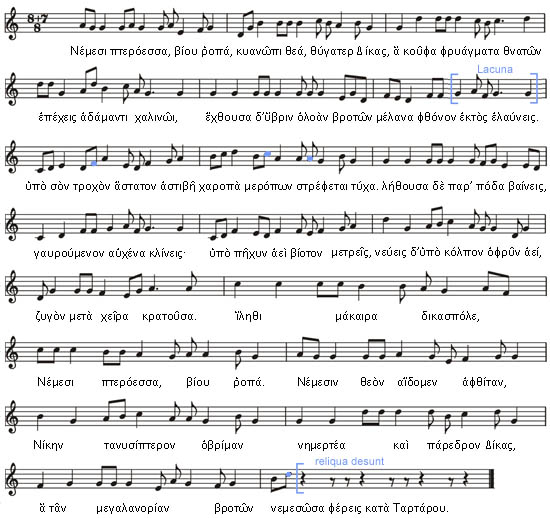
\includegraphics[scale=0.80]{ud-02/mes-hnem.jpg}
	\caption{Exemplo do himno a némesis}
	\label{nemesis-himno}
	\end{figure}
%
\begin{ejercicio}[Comentario resumo do \textit{Himno a Némesis}]
Identifica as características principais da audición.
% ESPACIO PARA REDACTAR O COMENTARIO DA AUDICIÓN
        \vspace*{3.3cm}
\end{ejercicio}
 

\newpage
%
% ACTIVIDADE 5.- 
%
%% EXERCICIOS PARA INCLUÍR DENTRO DO CADERNO DE EXERCICIOS %%
%
% EXERCICIO DE TRANSCRICIÓN: Epitafio de Seikilos.
%
\section{A notación musical na Antiga Grecia}


Dentro das fontes conservadas da cultura musical grega, existen aproximadamente sobre uns vinte exemplos, malia que tan só uns poucos son considerados realmente fiables, en parte debido a que a maioría deles non se conservan na súa totalidade. 

O máis destacable é un fragmento da obra de \textit{Orestes}, de Eurípides do 250 a.C., aproximadamente. Trátase dun \textit{stasimon}, isto é, un coro cantado na \textit{orchestra} (lugar diante do escenario, onde se colocaban algúns dos participantes na traxedia). A conservación é realmente boa, a pesares de non ser perfecta debido a que foi escrito en papiro e algunhas das partes perdéronse.

\subsection*{O Epitafio de Seikilos}

A fonte de información da cultura grega de maior importancia que se conserva, e que máis información aporta, é o \textit{skolion} (epitafio) de Seikilos, do século II a.C. aproximadamente. Escrito en pedra (nunha estela funeraria da actual Turquía conservado en Dinamarca), presenta unha magnífica conservación que permitiu descifralo totalmente. Podemos afirmar que é a obra máis coñecida da Antiga Grecia.

\subsubsection*{O texto}

Inscrita nunha columna (estela funeraria), serviu de epitafio a unha muller: na dedicatoria, Seikilos ofrece a unha muller (probablemente a súa esposa ou filla) unha canción, que aparece con notación musical e texto:

\begin{figure}[htp]
\centering
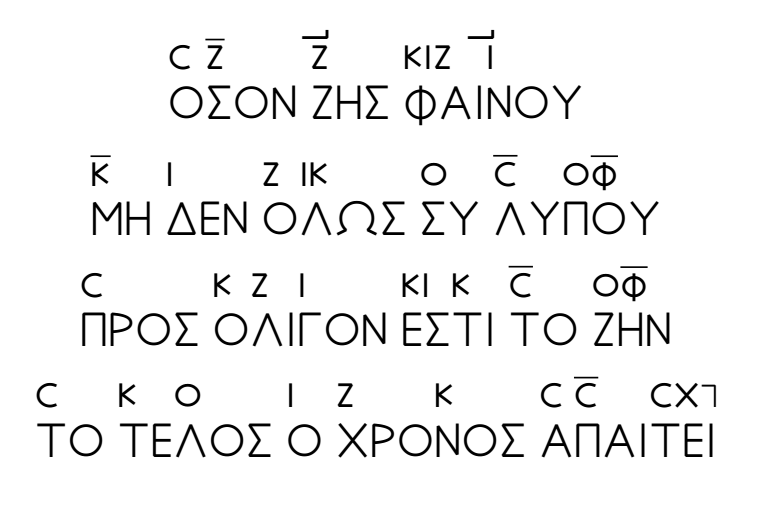
\includegraphics[scale=1.00]{ud-02/Seikilos-Ejercicio-03.png}
\caption{Texto do epitafio de Seikilos}
\label{Seikilos-texto}
\end{figure}

A tradución sería algo semellante a: \textit{ Mentres vivas, brilla; que nada te faga sufrir; a vida é moi curta e o tempo marca a fin.}

A achega máis destacable ou importante deste documento histórico aos estudos da música grega, foi sen dúbida a notación rítmica, que ao igual que a melódica, emprega signos do alfabeto grego. As notas sen indicación rítmica, valerían un pulso (\textit{chronos protos}), as sinaladas cun guión terían dous pulsos (\textit{diseme}); finalmente, as que levan guión cun sinal ou punto na parte superior dereita valerían tres pulsos (*\textit{triseme}).

\subsubsection*{A notación musical}

\begin{itemize}
\item Para indicar a altura dos sons, empregábase un signo diferente segundo cada altura. Os signos que aparecen nesta peza, ordenados de xeito ascendente son:

	\begin{figure}[htp]
	\centering
	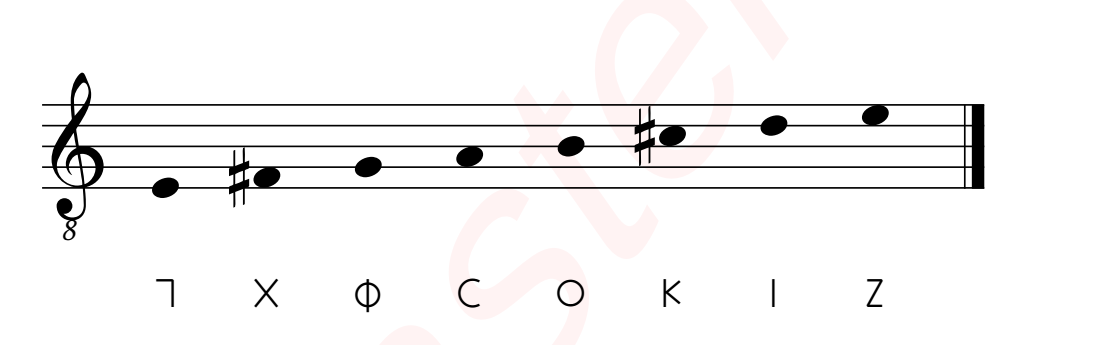
\includegraphics[scale=1.00]{ud-02/Seikilos-Ejercicio-01.png}
	\caption{Sitema de notación}
	\label{seikilos-sistema}
	\end{figure}
	
\item Para indicar a duración, empregábanse uns signos adicionais sobre os anteriores:
	\begin{figure}[htp]
	\centering
	
\includegraphics[scale=1.00]{ud-02/Seikilos-Ejercicio-02.png}
	\caption{Indicación da duración}
	\label{seikilos-duracion}
	\end{figure}
	
\end{itemize}

\subsubsection*{Transcrición}

Tendo en conta o indicado ata o de agora, realiza unha transcrición á notación actual da melodía do epitafio de Seikilos.

\begin{figure}[htp]
\centering
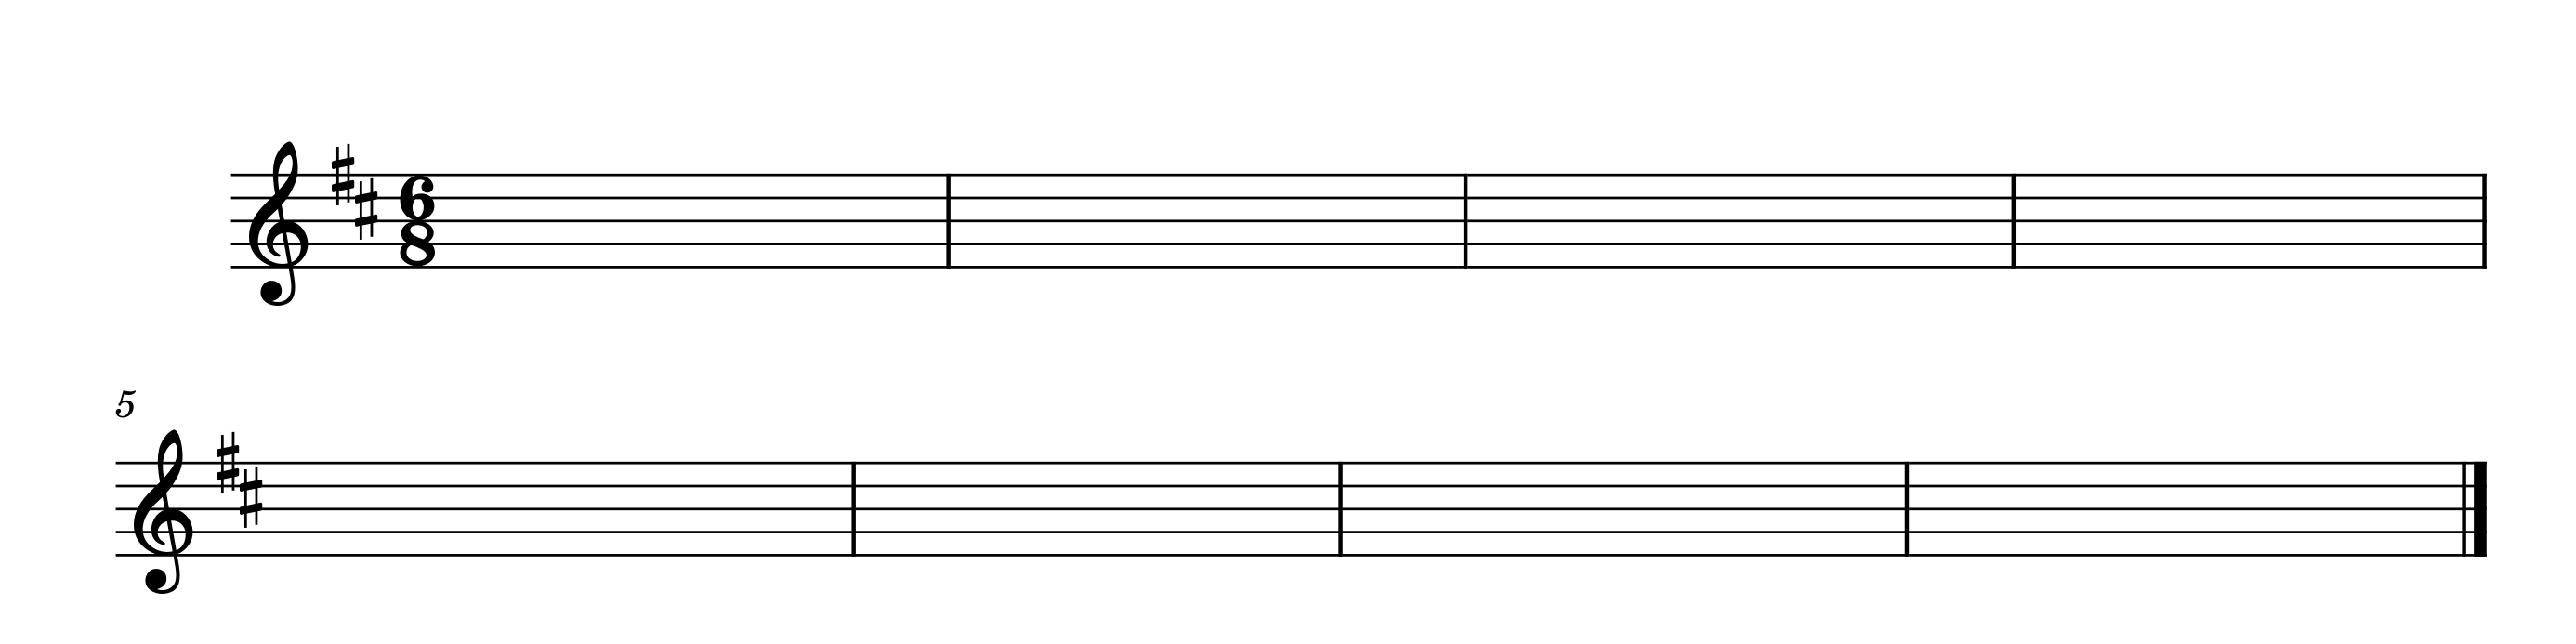
\includegraphics[scale=0.90]{ud-02/Seikilos-1.png}
\caption{Transcrición a notación moderna do epitadio de Seikilos}
\label{transcricion}
\end{figure}

\newpage
%
% ACTIVIDADE 6.- 
%
\begin{ejercicio}[Audición comentada \textit{Epitafio Seikilos}]
Le con atención a seguinte audición comentada do \textit{Epitafio de Seikilos}, fixándote nos diferentes aspectos que se comentan.
%
   \begin{enumerate}[1.-]

       \item \textbf{Contextualización}
       \par
O Epitafio de Seikilos é un fragmento de inscrición epigráfica grega achado nunha columna de mármore posta sobre a tumba que fixera construír Seikilos para a súa esposa Euterpe, preto de Trales (en Asia Menor).
\par
Conservada actualmente no Museo Nacional de Dinamarca, foi descuberta en 1883 por Sir W. M. Ramsay en Turquía e conservada no museo da antiga cidade de Esmirna. Durante o holocausto de Asia Menor (1919-1922), no que a cidade de Esmirna foi destruida, non se tivo coñecemento do seu paradeiro; posteriormente foi recuperada con sinais de desgaste e deterioro na súa base e coa última liña do texto borrada.
\par
Este manuscrito constitúe un exemplo de forma de composición musical grega, co engadido de ser a melodía escrita máis antiga que se coñece. A inscrición, contén un texto en grego sobre o que se desenvolve a melodía

   \item \textbf{Timbre} \par
A canción é melancólica, clasificada como \textit{skolion} ou "canción para beber".

    \item \textbf{Textura} \par
    \begin{itemize}
        \item 
        A composición está construída e organizada segundo principios modais.
        \item 
        Está en modo *Mixolidio actual e desenvólvese nun ámbito de oitava xusta. 
        \item
        Aparecen todos os sons da escala La4 + Mi5, con *Fa e *Do sostidos.
        \item
        O son que aparece con máis frecuencia é La4 (oito aparicións), seguido de Mi5 (seis aparicións). 
        \item
        O La4 é o son máis grave, que cerra a composición. 
        \item 
        O ámbito estreito, a escaseza de saltos e a (presumible) utilización dun instrumento para dobrar a liña vocal fan que interpretación a da melodía non revista complexidade técnica algunha.
    \end{itemize}

    \item \textbf{Melodía} \par
        \begin{itemize}
            \item 
            É de ámbito estreito: (a distancia entre a nota máis grave e a nota máis aguda é dunha oitava), que discorre sobre todo por graos conxuntos (intervalos de segunda e terceira).
            \item 
            Entre os saltos melódicos, só pode destacarse o de quinta ascendente co que se inicia a composición. 
            \item 
            A melodía está dividida en catro fases, exactamente iguais en duración (12 tempos cada unha). 
            \item 
            Todas as frases, excepto a última, terminan cun son prolongado, e todas as frases, excepto a primeira, poden considerarse cerradas.
        \end{itemize}
        
    \item \textbf{Ritmo} \par
    \begin{itemize}
        \item 
        Descoñécese a velocidade (tempo) da canción, xa que non está explicada na notación.
        \item 
        O tempo básico, ou unidade de duración (chronos protos), é a duración breve,transcrita en notación ortocrónica como corchea.
        \item
        Cada frase musical, e cada verso do poema, están constituídos por 12 *chronos protos. 
        \item 
        As tres últimas frases teñen unha construción rítmica moi semellante.
        \item
        Os sons da peza poden ter tres duracións: \begin{enumerate}
            \item 
            a trancrita como corchea (chronos protos),
            \item a transcrita como negra (diseme ou dúas chronos protos) e
            \item a negra con puntillo (triseme chronos protos).
            \end{enumerate}
    \end{itemize}

    \item \textbf{Forma} \par
        \begin{itemize}
            \item 
            Estamos ante unha composición que comeza con unha breve introdución de percusión, seguida da melodía principal introducida pola corda, que posteriormente realizará a voz. 
            Trátase dunha forma de reducidas dimensións con intervención da percusión, corda e voz; neste caso é unha forma menor e de ritmo libre seguindo as características da música da Grecia Clásica.
            \par
            
        \end{itemize}

    \item \textbf{Relación música texto}
        \begin{itemize}
            \item 
            A inscrición cantada, segundo a pronuncia do grego \textit{koiné}.
            \item 
            Como é característico da música da Grecia Antiga, melodía e texto forman un todo unificado.
            \item 
            Cada frase musical coincide con cada un dos catro versos que constitúen a composición literaria. 
            \item 
            A relación entre o texto e a música é de estilo silábica (sílaba por nota) con pequenos adornos.
        \end{itemize}     
        
   \end{enumerate}
\end{ejercicio}
\newpage

\newpage
%
\end{document}
%Fin de Hoja de ejercicios
%
